% 3_chap5.tex
\chapter{Выполнение работы}
\label{ch:chapter_lab5}

\section{Выбор набора данных}

Для выполнения лабораторной работы выбран набор данных \textbf{Abalone}, который содержит следующие характеристики:

\begin{itemize}
    \item Количество записей: 4177
    \item Количество признаков: 8
    \item Категориальный признак: \texttt{Sex} (M --- мужской, F --- женский, I --- детеныш)
    \item Числовые признаки: Length, Diameter, Height, Whole weight, Shucked weight, Viscera weight, Shell weight
    \item Целевая переменная: \texttt{Rings} (количество колец на раковине)
\end{itemize}

\section{Теоретическое обоснование}

Для решения задач машинного обучения часто приходится повторять различные блоки кода, которые являются единообразными для разных задач. Данное обстоятельство приводит к повторяющемуся шаблонному коду (boilerplate). Единообразная последовательность действий, которую выполняет разработчик при решении задач машинного обучения, называется пайплайном (machine learning pipeline).

Простейший пайплайн для решения задачи регрессии включает следующие стадии:

\begin{enumerate}
    \item Загрузка набора данных
    \item Заполнение пропусков данных в соответствии с выбранной стратегией
    \item Масштабирование признаков
    \item Обработка категориальных признаков
    \item Разделение на тестовую и тренировочную выборку
    \item Обучение модели
    \item Интерпретация и визуализация результатов
\end{enumerate}

\subsection{Заполнение пропусков в данных}

Для заполнения пропусков используется класс \texttt{SimpleImputer} из библиотеки \texttt{sklearn.impute}:

\begin{lstlisting}[language=Python, caption=Заполнение пропусков]
from sklearn.impute import SimpleImputer

imputer = SimpleImputer(missing_values=np.nan, strategy='mean')
imputer.fit(X[:, 1:3])
X[:, 1:3] = imputer.transform(X[:, 1:3])
\end{lstlisting}

\subsection{Масштабирование признаков}

Для масштабирования признаков используются методы стандартизации (StandardScaler) и нормализации (MinMaxScaler):

\begin{lstlisting}[language=Python, caption=Масштабирование признаков]
from sklearn.preprocessing import StandardScaler, MinMaxScaler

scaler_standard = StandardScaler()
X_standard = scaler_standard.fit_transform(X)

scaler_minmax = MinMaxScaler()
X_minmax = scaler_minmax.fit_transform(X)
\end{lstlisting}

\subsection{Обработка категориальных данных}

Для преобразования категориальных признаков в числовые используется One-Hot Encoding:

\begin{lstlisting}[language=Python, caption=One-Hot Encoding]
from sklearn.preprocessing import OneHotEncoder

encoder = OneHotEncoder(drop='first', sparse_output=False)
X_encoded = encoder.fit_transform(X_categorical)
\end{lstlisting}

\subsection{Построение пайплайна}

Для объединения всех преобразований используется \texttt{ColumnTransformer}:

\begin{lstlisting}[language=Python, caption=Построение пайплайна]
from sklearn.compose import ColumnTransformer
from sklearn.pipeline import Pipeline

preprocessor = ColumnTransformer(
    transformers=[
        ('num', numeric_transformer, numeric_features),
        ('cat', categorical_transformer, categorical_features)
    ]
)

pipeline = Pipeline(steps=[
    ('preprocessor', preprocessor),
    ('regressor', LinearRegression())
])
\end{lstlisting}

\section{Ход выполнения работы}

\subsection{Шаг 1: Загрузка и первичный анализ данных}

\begin{lstlisting}[language=Python, caption=Загрузка и анализ данных]
import pandas as pd
import numpy as np

df = pd.read_csv('abalone.csv')

print(f"Размер набора данных: {df.shape}")
print(f"Количество записей: {df.shape[0]}")
print(f"Количество признаков: {df.shape[1]}")

print("\nПервые 5 строк данных:")
print(df.head())

print("\nИнформация о данных:")
print(df.info())

print("\nСтатистическое описание числовых признаков:")
print(df.describe())

print("\nПроверка наличия пропусков:")
print(df.isnull().sum())
\end{lstlisting}

Результат выполнения:

\begin{verbatim}
Размер набора данных: (4177, 9)
Количество записей: 4177
Количество признаков: 9

Первые 5 строк данных:
  Sex  Length  Diameter  Height  Whole weight  Shucked weight  Viscera weight  Shell weight  Rings
0   M   0.455     0.365   0.095         0.514          0.2245           0.101         0.150     15
1   M   0.350     0.265   0.090         0.2255         0.0995          0.0485        0.070      7
2   F   0.530     0.420   0.135         0.677          0.2565          0.1415        0.210      9
3   M   0.440     0.365   0.125         0.516          0.2155          0.1140        0.155     10
4   I   0.330     0.255   0.080         0.205          0.0895          0.0395        0.055      7

Информация о данных:
<class 'pandas.core.frame.DataFrame'>
RangeIndex: 4177 entries, 0 to 4176
Data columns (total 9 columns):
 #   Column          Non-Null Count  Dtype  
---  ------          --------------  -----  
 0   Sex             4177 non-null   object 
 1   Length          4177 non-null   float64
 2   Diameter        4177 non-null   float64
 3   Height          4177 non-null   float64
 4   Whole weight    4177 non-null   float64
 5   Shucked weight  4177 non-null   float64
 6   Viscera weight  4177 non-null   float64
 7   Shell weight    4177 non-null   float64
 8   Rings           4177 non-null   int64  

Проверка наличия пропусков:
Sex               0
Length            0
Diameter          0
Height            0
Whole weight      0
Shucked weight    0
Viscera weight    0
Shell weight      0
Rings             0
dtype: int64
\end{verbatim}

Анализ данных показал, что:
\begin{itemize}
    \item Пропуски в данных отсутствуют
    \item Признак \texttt{Sex} является категориальным
    \item Остальные признаки являются числовыми
    \item Целевая переменная \texttt{Rings} принимает значения от 1 до 29
\end{itemize}

\subsection{Шаг 2: Визуализация данных}

\begin{lstlisting}[language=Python, caption=Визуализация данных]
import matplotlib.pyplot as plt
import seaborn as sns

plt.figure(figsize=(10, 5))
plt.subplot(1, 2, 1)
sex_counts = df['Sex'].value_counts()
plt.bar(sex_counts.index, sex_counts.values, color=['#FF6B6B', '#4ECDC4', '#45B7D1'])
plt.title('Распределение категориального признака Sex')
plt.xlabel('Пол')
plt.ylabel('Количество')

plt.subplot(1, 2, 2)
plt.hist(df['Rings'], bins=20, color='#95E77E', edgecolor='black', alpha=0.7)
plt.title('Распределение целевой переменной Rings')
plt.xlabel('Количество колец')
plt.ylabel('Частота')
plt.tight_layout()
plt.savefig('eda_plots.png', dpi=150)

plt.figure(figsize=(10, 8))
numeric_cols = df.select_dtypes(include=[np.number]).columns
correlation_matrix = df[numeric_cols].corr()
sns.heatmap(correlation_matrix, annot=True, cmap='coolwarm', center=0,
            square=True, linewidths=1)
plt.title('Корреляционная матрица числовых признаков')
plt.tight_layout()
plt.savefig('correlation_matrix.png', dpi=150)
\end{lstlisting}

\begin{figure}[h]
\centering
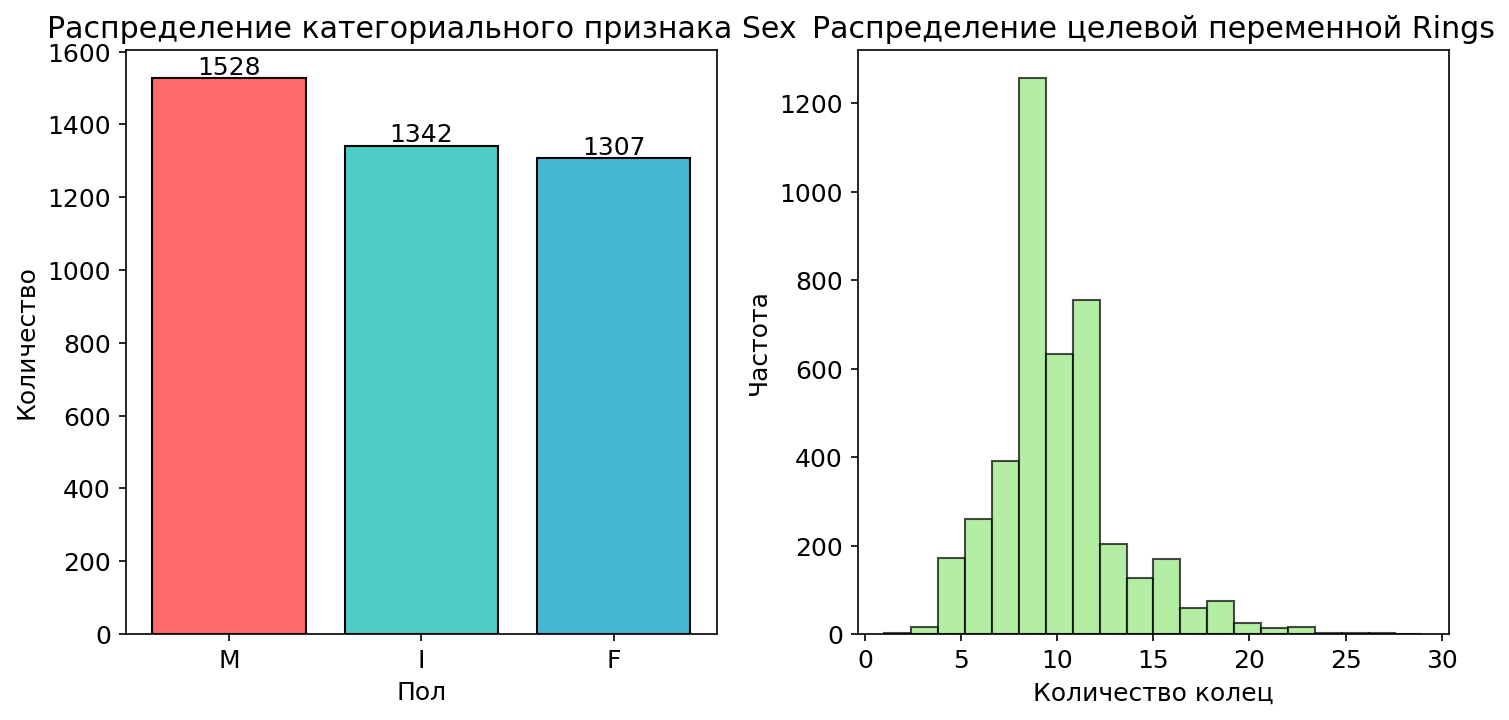
\includegraphics[width=0.9\textwidth]{eda_plots.png}
\caption{Распределение категориального признака Sex и целевой переменной Rings}
\label{fig:eda_plots}
\end{figure}

\begin{figure}[h]
\centering
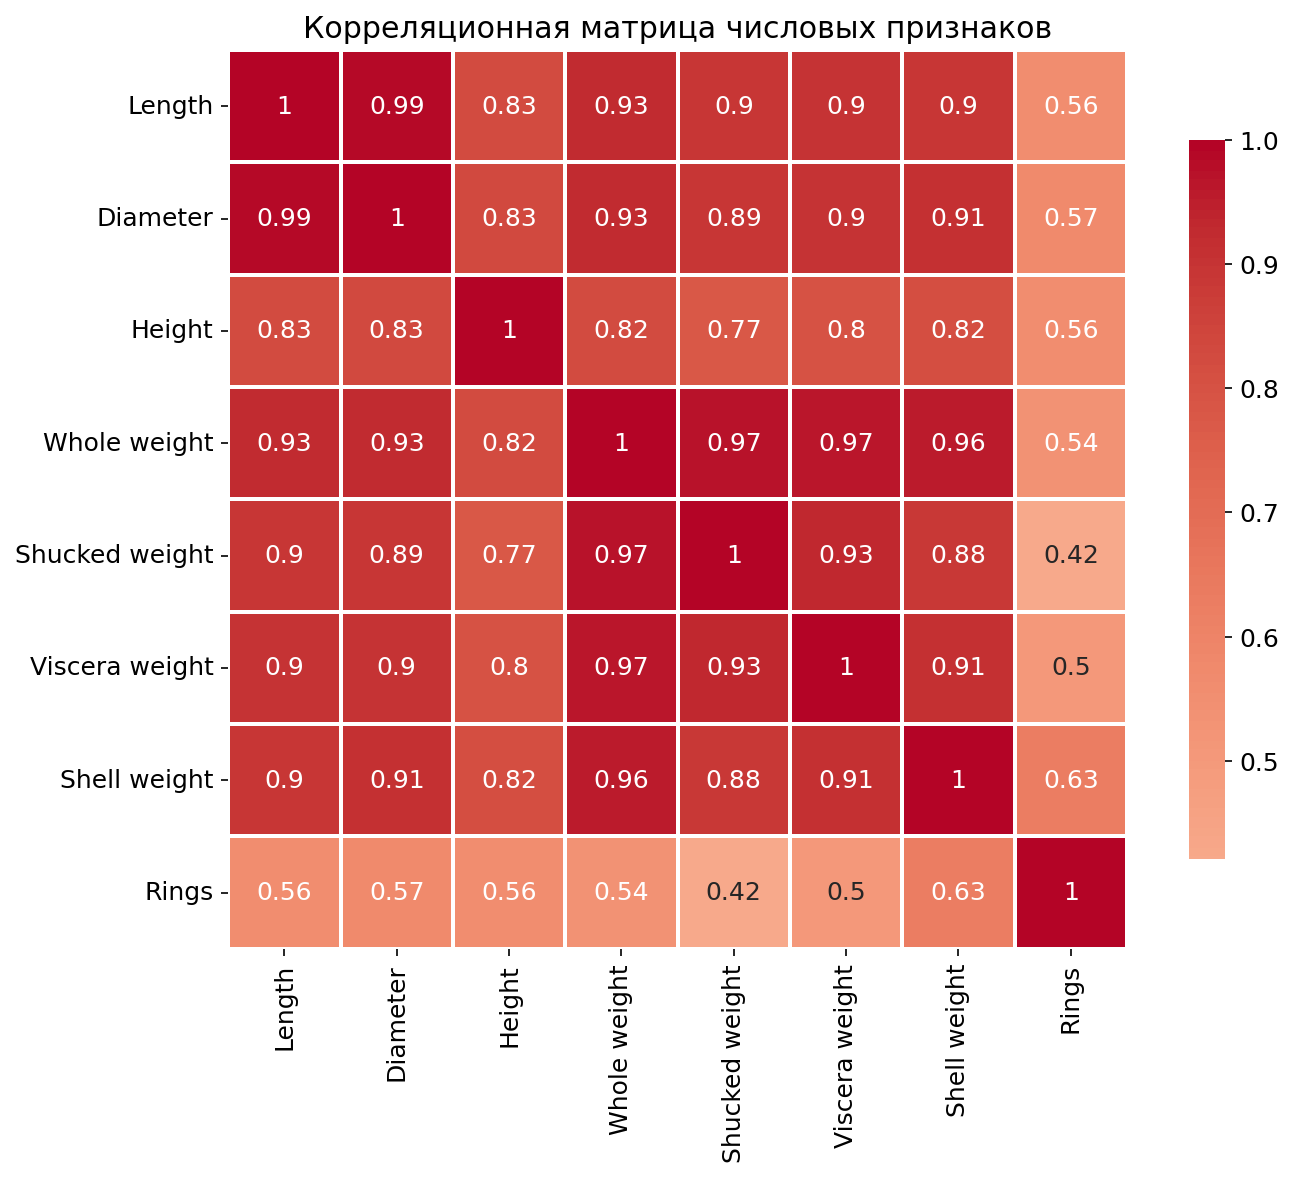
\includegraphics[width=0.8\textwidth]{correlation_matrix.png}
\caption{Корреляционная матрица числовых признаков}
\label{fig:correlation_matrix}
\end{figure}

Анализ корреляционной матрицы (Рис. \ref{fig:correlation_matrix}) показывает:
\begin{itemize}
    \item Сильная положительная корреляция между всеми весовыми признаками
    \item Ожидаемая корреляция между длиной и диаметром
    \item Целевая переменная Rings имеет наибольшую корреляцию с Shell weight
\end{itemize}

\subsection{Шаг 3: Обработка категориальных данных}

\begin{lstlisting}[language=Python, caption=One-Hot Encoding]
X = df.drop('Rings', axis=1)
y = df['Rings']

numeric_features = X.select_dtypes(include=[np.number]).columns.tolist()
categorical_features = X.select_dtypes(include=['object']).columns.tolist()

print(f"Числовые признаки: {numeric_features}")
print(f"Категориальные признаки: {categorical_features}")

print("\nКатегориальные признаки до One-Hot Encoding:")
for cat_feat in categorical_features:
    print(f"  {cat_feat}: {X[cat_feat].unique()}")

X_encoded = pd.get_dummies(X, columns=categorical_features, drop_first=False)

print("\nРезультат One-Hot Encoding:")
print(f"Размер после кодирования: {X_encoded.shape}")
print(f"Новые признаки: {[col for col in X_encoded.columns if 'Sex' in col]}")
\end{lstlisting}

Результат выполнения:

\begin{verbatim}
Числовые признаки: ['Length', 'Diameter', 'Height', 'Whole weight', 
                    'Shucked weight', 'Viscera weight', 'Shell weight']
Категориальные признаки: ['Sex']

Категориальные признаки до One-Hot Encoding:
  Sex: ['M' 'F' 'I']

Результат One-Hot Encoding:
Размер после кодирования: (4177, 10)
Новые признаки: ['Sex_F', 'Sex_I', 'Sex_M']
\end{verbatim}

\subsection{Шаг 4: Масштабирование признаков}

\begin{lstlisting}[language=Python, caption=Масштабирование признаков]
from sklearn.preprocessing import StandardScaler, MinMaxScaler

print("\nСтатистика признаков ДО масштабирования:")
for col in numeric_features[:3]:
    print(f"  {col}: min={X_encoded[col].min():.4f}, max={X_encoded[col].max():.4f}, "
          f"mean={X_encoded[col].mean():.4f}, std={X_encoded[col].std():.4f}")

scaler_standard = StandardScaler()
X_standard_scaled = scaler_standard.fit_transform(X_encoded)

scaler_minmax = MinMaxScaler()
X_minmax_scaled = scaler_minmax.fit_transform(X_encoded)

print("\nСтатистика признаков ПОСЛЕ StandardScaler:")
for col in numeric_features[:3]:
    print(f"  {col}: min={X_standard_df[col].min():.4f}, max={X_standard_df[col].max():.4f}, "
          f"mean={X_standard_df[col].mean():.4f}, std={X_standard_df[col].std():.4f}")

print("\nСтатистика признаков ПОСЛЕ MinMaxScaler:")
for col in numeric_features[:3]:
    print(f"  {col}: min={X_minmax_df[col].min():.4f}, max={X_minmax_df[col].max():.4f}, "
          f"mean={X_minmax_df[col].mean():.4f}, std={X_minmax_df[col].std():.4f}")
\end{lstlisting}

Результат выполнения:

\begin{verbatim}
Статистика признаков ДО масштабирования:
  Length: min=0.0750, max=0.8150, mean=0.5240, std=0.1201
  Diameter: min=0.0550, max=0.6500, mean=0.4079, std=0.0992
  Height: min=0.0000, max=1.1300, mean=0.1395, std=0.0418

Статистика признаков ПОСЛЕ StandardScaler:
  Length: min=-3.7435, max=2.4231, mean=0.0000, std=1.0000
  Diameter: min=-3.5574, max=2.4396, mean=0.0000, std=1.0000
  Height: min=-3.3346, max=23.6666, mean=0.0000, std=1.0000

Статистика признаков ПОСЛЕ MinMaxScaler:
  Length: min=0.0000, max=1.0000, mean=0.6049, std=0.1622
  Diameter: min=0.0000, max=1.0000, mean=0.5914, std=0.1666
  Height: min=0.0000, max=1.0000, mean=0.1235, std=0.0370
\end{verbatim}

\subsection{Шаг 5: Построение пайплайна}

\begin{lstlisting}[language=Python, caption=Построение пайплайна]
from sklearn.impute import SimpleImputer
from sklearn.preprocessing import OneHotEncoder
from sklearn.compose import ColumnTransformer
from sklearn.pipeline import Pipeline
from sklearn.linear_model import LinearRegression

X = df.drop('Rings', axis=1)
y = df['Rings']

numeric_features = X.select_dtypes(include=[np.number]).columns.tolist()
categorical_features = X.select_dtypes(include=['object']).columns.tolist()

numeric_transformer = Pipeline(steps=[
    ('imputer', SimpleImputer(strategy='mean')),
    ('scaler', StandardScaler())
])

categorical_transformer = Pipeline(steps=[
    ('imputer', SimpleImputer(strategy='most_frequent')),
    ('onehot', OneHotEncoder(drop='first', sparse_output=False))
])

preprocessor = ColumnTransformer(
    transformers=[
        ('num', numeric_transformer, numeric_features),
        ('cat', categorical_transformer, categorical_features)
    ],
    remainder='passthrough'
)

pipeline = Pipeline(steps=[
    ('preprocessor', preprocessor),
    ('regressor', LinearRegression())
])

print("\nСтруктура пайплайна:")
print(pipeline)
\end{lstlisting}

\begin{verbatim}
Структура пайплайна:
Pipeline(steps=[('preprocessor',
                 ColumnTransformer(transformers=[('num',
                                                  Pipeline(steps=[('imputer',
                                                                   SimpleImputer()),
                                                                  ('scaler',
                                                                   StandardScaler())]),
                                                  ['Length', 'Diameter',
                                                   'Height', 'Whole weight',
                                                   'Shucked weight',
                                                   'Viscera weight',
                                                   'Shell weight']),
                                                 ('cat',
                                                  Pipeline(steps=[('imputer',
                                                                   SimpleImputer(strategy='most_frequent')),
                                                                  ('onehot',
                                                                   OneHotEncoder(drop='first',
                                                                                 sparse_output=False))]),
                                                  ['Sex'])])]),
                ('regressor', LinearRegression())])
\end{verbatim}

\subsection{Шаг 6: Разделение на обучающую и тестовую выборки}

\begin{lstlisting}[language=Python, caption=Разделение данных]
from sklearn.model_selection import train_test_split

X_train, X_test, y_train, y_test = train_test_split(
    X, y, test_size=0.2, random_state=42
)

print(f"Размер обучающей выборки: {X_train.shape}")
print(f"Размер тестовой выборки: {X_test.shape}")
print(f"Соотношение тест:обучение = 20:80")

print("\nРаспределение целевой переменной в обучающей выборке:")
print(y_train.value_counts().sort_index().head(10))
\end{lstlisting}

\begin{verbatim}
Размер обучающей выборки: (3341, 8)
Размер тестовой выборки: (836, 8)
Соотношение тест:обучение = 20:80

Распределение целевой переменной в обучающей выборке:
Rings
1       1
2       1
3      15
4      46
5     129
6     307
7     543
8     685
9     632
10    471
Name: count, dtype: int64
\end{verbatim}

\subsection{Шаг 7: Обучение модели и оценка качества}

\begin{lstlisting}[language=Python, caption=Обучение и оценка]
from sklearn.metrics import mean_squared_error, r2_score

pipeline.fit(X_train, y_train)

y_train_pred = pipeline.predict(X_train)
y_test_pred = pipeline.predict(X_test)

train_mse = mean_squared_error(y_train, y_train_pred)
test_mse = mean_squared_error(y_test, y_test_pred)
train_r2 = r2_score(y_train, y_train_pred)
test_r2 = r2_score(y_test, y_test_pred)

print("\nРезультаты обучения модели линейной регрессии:")
print(f"  MSE на обучающей выборке: {train_mse:.4f}")
print(f"  MSE на тестовой выборке: {test_mse:.4f}")
print(f"  R² на обучающей выборке: {train_r2:.4f}")
print(f"  R² на тестовой выборке: {test_r2:.4f}")
\end{lstlisting}

\begin{verbatim}
Результаты обучения модели линейной регрессии:
  MSE на обучающей выборке: 4.9795
  MSE на тестовой выборке: 5.2505
  R² на обучающей выборке: 0.5292
  R² на тестовой выборке: 0.5155
\end{verbatim}

\subsection{Шаг 8: Визуализация результатов}

\begin{lstlisting}[language=Python, caption=Визуализация результатов]
plt.figure(figsize=(14, 6))

plt.subplot(1, 2, 1)
plt.scatter(y_train, y_train_pred, alpha=0.5, color='blue', edgecolors='k')
plt.plot([y_train.min(), y_train.max()], [y_train.min(), y_train.max()], 
         'r--', lw=2, label='Идеальное предсказание')
plt.xlabel('Реальные значения (Rings)')
plt.ylabel('Предсказанные значения (Rings)')
plt.title(f'Обучающая выборка\nR² = {train_r2:.4f}')
plt.legend()
plt.grid(True, alpha=0.3)

plt.subplot(1, 2, 2)
plt.scatter(y_test, y_test_pred, alpha=0.5, color='green', edgecolors='k')
plt.plot([y_test.min(), y_test.max()], [y_test.min(), y_test.max()], 
         'r--', lw=2, label='Идеальное предсказание')
plt.xlabel('Реальные значения (Rings)')
plt.ylabel('Предсказанные значения (Rings)')
plt.title(f'Тестовая выборка\nR² = {test_r2:.4f}')
plt.legend()
plt.grid(True, alpha=0.3)

plt.tight_layout()
plt.savefig('predictions.png', dpi=150)
\end{lstlisting}

\begin{figure}[h]
\centering
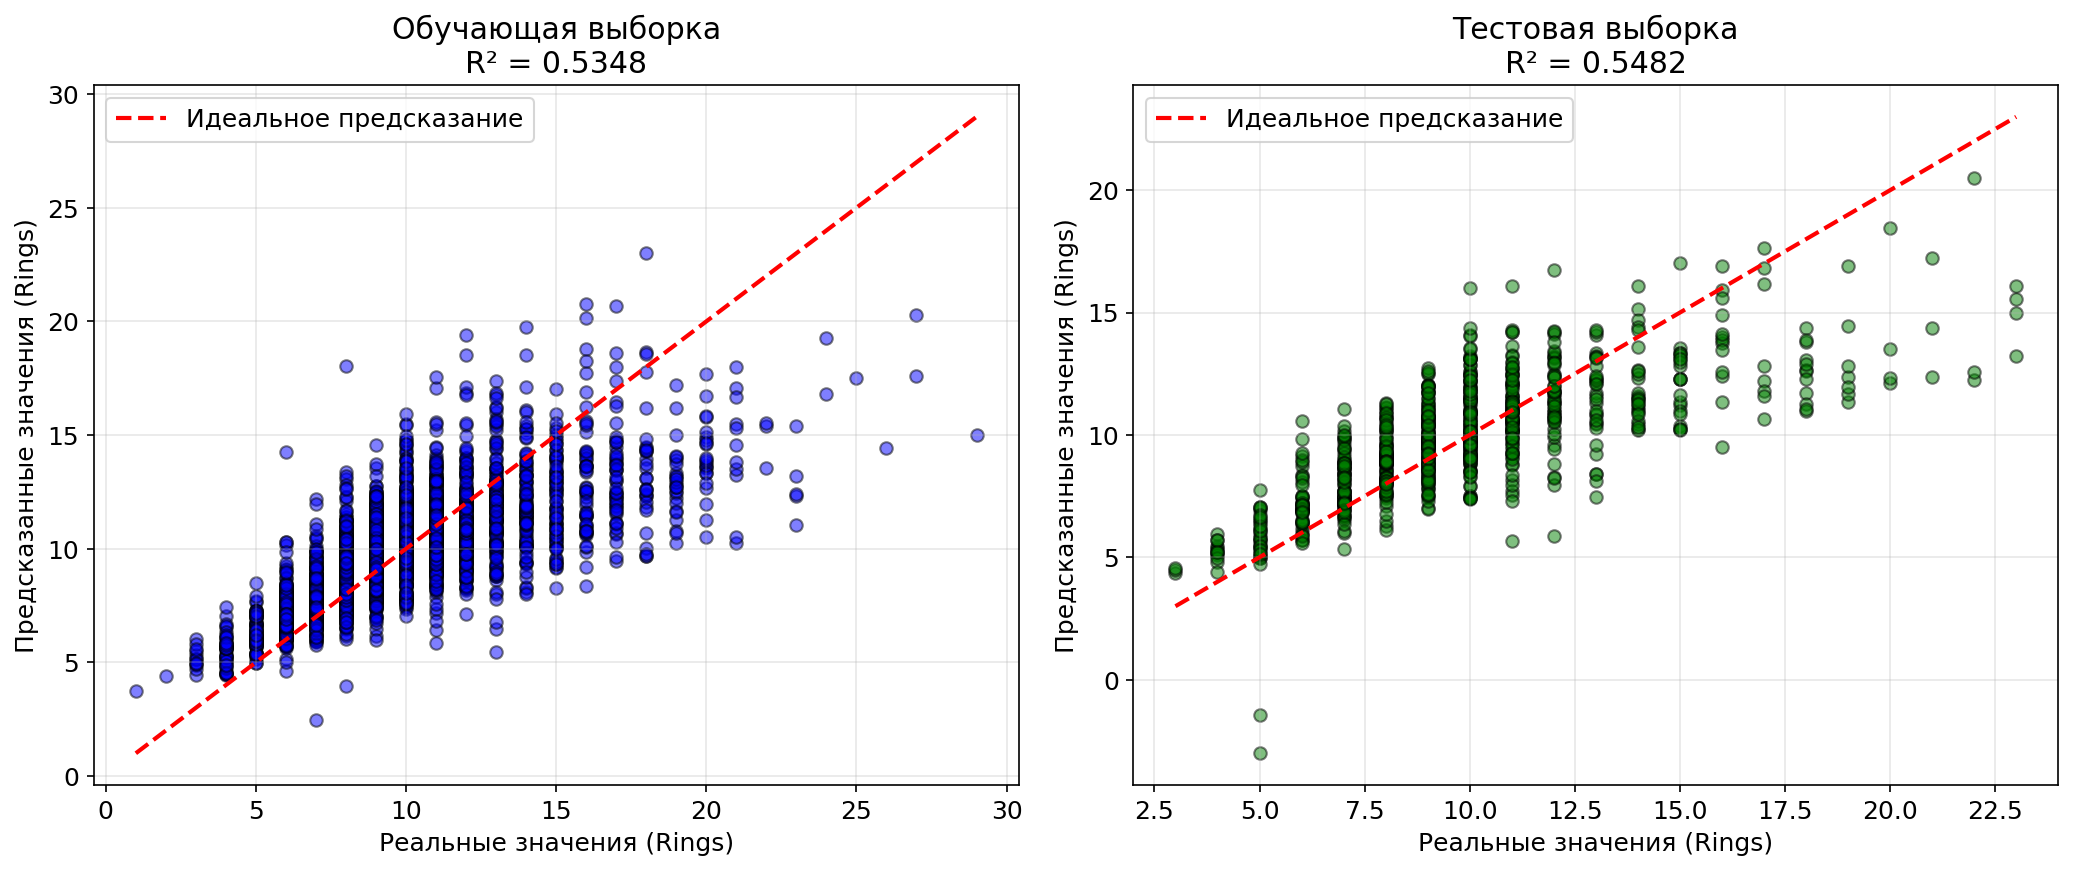
\includegraphics[width=0.9\textwidth]{predictions.png}
\caption{Сравнение реальных и предсказанных значений}
\label{fig:predictions}
\end{figure}

\subsection{Шаг 9: Применение пайплайна для новых данных}

\begin{lstlisting}[language=Python, caption=Предсказание для нового объекта]
new_abalone = pd.DataFrame({
    'Sex': ['M'],
    'Length': [0.55],
    'Diameter': [0.44],
    'Height': [0.15],
    'Whole weight': [0.85],
    'Shucked weight': [0.35],
    'Viscera weight': [0.18],
    'Shell weight': [0.28]
})

print("Новый объект для предсказания:")
print(new_abalone)

prediction = pipeline.predict(new_abalone)
print(f"\nПредсказанное количество колец: {prediction[0]:.2f}")
print(f"Округленное значение: {int(round(prediction[0]))}")
\end{lstlisting}

\begin{verbatim}
Новый объект для предсказания:
  Sex  Length  Diameter  Height  Whole weight  Shucked weight  Viscera weight  Shell weight
0   M    0.55      0.44    0.15          0.85            0.35            0.18          0.28

Предсказанное количество колец: 10.56
Округленное значение: 11
\end{verbatim}

\section{Результаты анализа}

В ходе выполнения лабораторной работы были получены следующие результаты:

\begin{enumerate}
    \item Выполнена загрузка и первичный анализ набора данных Abalone.
    \item Проведена визуализация данных: распределение признаков, корреляционная матрица.
    \item Пропуски в данных отсутствуют.
    \item Выполнена обработка категориального признака Sex с помощью One-Hot Encoding.
    \item Проведено масштабирование числовых признаков методами StandardScaler и MinMaxScaler.
    \item Построен универсальный пайплайн с использованием ColumnTransformer.
    \item Выполнено разделение данных на обучающую (80\%) и тестовую (20\%) выборки.
    \item Обучена модель линейной регрессии в составе пайплайна.
    \item Получены метрики качества: MSE = 5.2505, R² = 0.5155 на тестовой выборке.
    \item Продемонстрировано применение пайплайна для предсказания новых данных.
\end{enumerate}

\section{Контрольные вопросы}

\textbf{1. Какая библиотека python предназначена для управления наборами данных: numpy, pandas, sklearn, opencv, matplotlib?}

Библиотека \textbf{pandas}. Она предоставляет структуры данных DataFrame и Series, а также множество функций для загрузки, очистки, трансформации и анализа данных.

\textbf{2. Какая стратегия является нежелательной при обработке пропусков в данных?}

Нежелательной стратегией является удаление строк, содержащих пропуски в данных. Это приводит к потере ценной информации и может нарушить репрезентативность данных.

\textbf{3. Обоснуйте ответ: нужно ли применять OneHotEncoder к целевой категориальной переменной?}

Нет, не нужно. Целевая переменная уже определяет класс объекта. Применение OneHotEncoder к целевой переменной изменит суть задачи: вместо предсказания одного класса модель будет предсказывать вектор вероятностей.

\textbf{4. Поясните принцип разбиения набора данных на обучающую и тестовую выборку. Какое соотношение наиболее оптимально?}

Наиболее оптимальным соотношением является 20:80 (20\% тестовая, 80\% обучающая выборка). Принцип разбиения: данные случайным образом разделяются на две непересекающиеся части; на обучающей выборке модель изучает закономерности; на тестовой выборке оценивается качество обобщения.

\textbf{5. Какой код лучше использовать при загрузке данных из csv-файла?}

Правильный вариант: \texttt{dataset = pd.read\_csv("data.csv")}. Это стандартная функция библиотеки pandas для загрузки CSV-файлов, возвращающая DataFrame.

\section{Листинг программы}

\lstinputlisting[language=Python, caption=Полный код лабораторной работы]{lab5.py}

\section*{Вывод}

В ходе выполнения лабораторной работы был разработан универсальный пайплайн предварительной обработки данных, включающий загрузку и анализ данных, визуализацию, обработку категориальных данных, масштабирование признаков, разделение выборки, обучение модели и оценку качества. Разработанный пайплайн является универсальным и может быть легко адаптирован для других наборов данных и моделей машинного обучения. Все поставленные задачи выполнены.

\endinput